\documentclass[SoftwareDesign/SoftwareDesign_main.tex]{subfiles}

\documentclass{article}

\begin{document}
\section{Design av Car Profile Page}
Dette avsnittet presenterer designet av Viewet og den tilhørende ViewModelen til CarProfilePage. Den er designet med ViewFirst prinsippet på samme måte som HeaderBar.
\subsection{Design av View til Car Profile Page}
Designet for CarProfilePage er basert på en WireFrame som ble laget for siden, denne kan sees på figur \ref{fig:CarProfileWireframe}.

\begin{figure}[H]
    \centering
    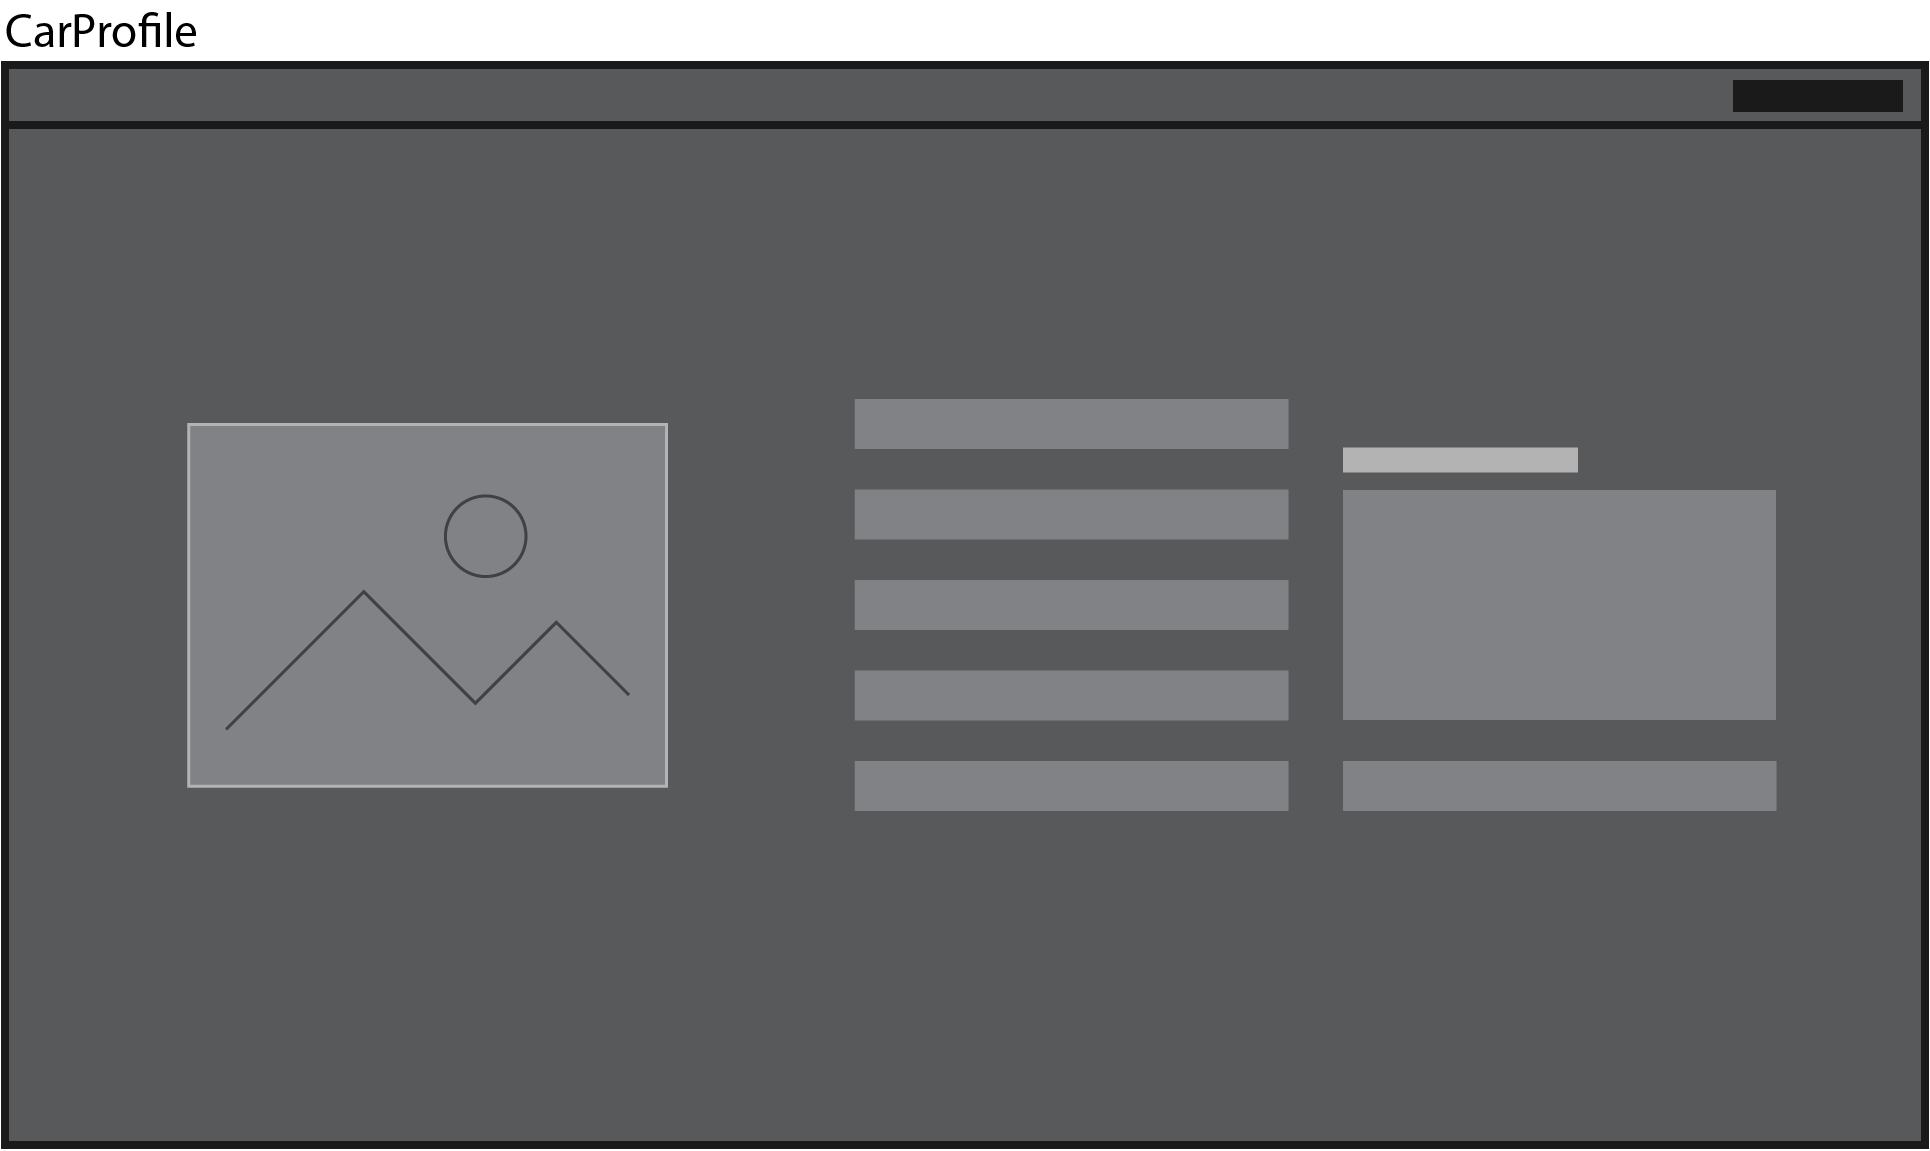
\includegraphics[width=\textwidth]{SoftwareDesign/MVVMDesigns/Graphics/CarProfileWireFrame.png}
    \caption{Car Profile WireFrame}
    \label{fig:CarProfileWireframe}
\end{figure}


CarProfile er siden man blir tatt til når man bestemmer seg for å leie ut bilen sin derfor skal den ha flere felter hvor brukeren kan inntaste informasjonen om bilen sin blant annet merke, modell og års nummer samt et sted hvor det kan lastes opp et bilde av bilen. Dette er også siden hvor brukeren kan bestemme hvilket tidsintervall bilen skal leies ut i. Denne siden blir også brukt som en side hvor utleieren kan se og redigere sin bil profil i ettertid.

\subsection{Design av ViewModel til CarProfile}
Funksjonaliteten til CarProfile vil variere etter om den skal brukes til å registrere en bil for første gang eller om utleieren skal redigere noe av informasjonen som er lagret om bilen.
\\
\\
Hvis det er en ny bil som skal registreres vil siden starte i edit mode. Hvor det så er redigerbare felter, en knapp hvor brukeren kan laste opp et bilde og en save knapp. Hvis brukeren skal se/redigere en allerede eksisterende bil vil en read only versjon av siden åpnes hvor det viser en knapp hvor det står edit.
\\
\\
\textbf{Edit knappen:}\\
Edit knappen er den eneste kappen som blir presentert til brukeren da han åpner Car Profile siden. Denne vil låse opp feltene og gjøre det mulig å redigere dem. I tilleg vil knappen endre seg til en save knapp.
\\
\\
\textbf{Save knappen:}\\
Save knappen sitt ansvar er å låse siden for videre redigering og samtidig oppdatere CarProfilen som ligger i databasen.
\\
\\
\textbf{Upload photo:}\\
Upload photo knappen åpner en ny dialog boks hvor man skal velge det nye bilde til bilen din. Dette bildet blir lagret som et BitmapImage i applikasonen og blir konvertert til en string når det overføres til databasen for lagring.




\end{document}